\documentclass{article}

\usepackage[english]{babel}
\usepackage[a4paper,top=2cm,bottom=2cm,left=3cm,right=3cm,marginparwidth=1.75cm]{geometry}
\usepackage{amsmath}
\usepackage{graphicx}
\usepackage[colorlinks=true, allcolors=blue]{hyperref}
\usepackage{subcaption}
\usepackage{placeins}
\usepackage{xspace}
\usepackage[us,24hr]{datetime}
\usepackage{helvet}
\renewcommand{\familydefault}{\sfdefault}
\usepackage{fp}
\usepackage{footnote}
\makesavenoteenv{tabular}

% input variables
\newcommand{\filemeas}{dipole\_2450MHz\_Flat\_10mm\_16.5dBm.csv}
\newcommand{\powerlevel}{16.5} % dBm
\newcommand{\noiselevel}{0.02} % W/kg

\newcommand{\antennatype}{dipole}
\newcommand{\frequency}{2450} % MHz
\newcommand{\distance}{10} % mm
\newcommand{\mass}{10}  % grams

\newcommand{\pssarref}{24.71}  % W/kg
\newcommand{\pssarmeas}{24.63} % W/kg
\newcommand{\errscale}{-0.35} % percent

\newcommand{\deltadist}{2~mm\xspace}
\newcommand{\deltadose}{5.0~\%\xspace}
\def\passrate{100.0}
\FPeval{\failrate}{round(100.0-\passrate,1)}

\FPiflt{\passrate}{100.0}%
    \newcommand{\passfail}{\textbf{Fail}}
    \newcommand{\statement}{The pattern validation fails because $\Gamma (x_e,y_e)~>~1.0$ for \failrate \% of the measured sSAR values, $sSAR_{en}(x_e,y_e)$, compared to the reference, $sSAR_{rn}(x'_r,y'_r)$, }
\else
    \newcommand{\passfail}{\textbf{Pass}}
    \newcommand{\statement}{The pattern validation passes because $\Gamma (x_e,y_e)~>~1.0$ for all of the measured sSAR values, $sSAR_{en}(x_e,y_e)$, compared to the reference, $sSAR_{rn}(x'_r,y'_r)$, }
\fi

\title{SAR Pattern Validation Report}

\begin{document}
\thispagestyle{empty}
\begin{center}
    \section*{SAR Pattern Validation Report for IEC/IEEE PAS 62209-5}
    \today
\end{center}

\subsection*{Measured sSAR Parameters}

File name with measurement, $sSAR_{en}(x_e,y_e)$: \texttt{\filemeas}

\begin{table}[htpb] \centering
\begin{tabular}{cccccc|ccc}
\textbf{Power} & \textbf{Noise} & \textbf{Source} &&& \textbf{Avg.}&\multicolumn{2}{c}{\textbf{psSAR at 30~dBm}}& \textbf{Sampling} \\
\textbf{Level} & \textbf{Level} &\textbf{Type} & \textbf{Freq.} & \textbf{Dist.} & \textbf{Mass} & \textbf{Measured} & \textbf{Reference} & \textbf{Error} \\
\textbf{(dBm)} & \textbf{(W/kg)} & & \textbf{(MHz)} & \textbf{(mm)} & \textbf{(g)} & \textbf{(W/kg)} & \textbf{(W/kg)} & \textbf{(\%)} \\\hline
\powerlevel & \noiselevel & \antennatype & \frequency & \distance & \mass & \pssarmeas & \pssarref & \errscale \\
\end{tabular}
\label{tab:meas-params}
\end{table}

\FloatBarrier
\subsection*{Pattern Match Result: \passfail}

\statement ~according to the Gamma criterion\footnote{
\[
\Gamma (x_e, y_e) = \min_{x'_r,y'_r}\Bigg(\sqrt{\frac{(x_e-x'_r)^2+(y_e-y'_r)^2}{\Delta d^2}+\frac{(sSAR_{en}(x_e,y_e)-sSAR_{rn}(x'_r,y'_r))^2}{\Delta D^2}}\Bigg)
\]
} with $\Delta D = $\deltadose, $\Delta d$ = \deltadist. See IEC/IEEE PAS 62209-5 for details.

\begin{figure}[h!]
  \centering
  \begin{tabular}{c}
    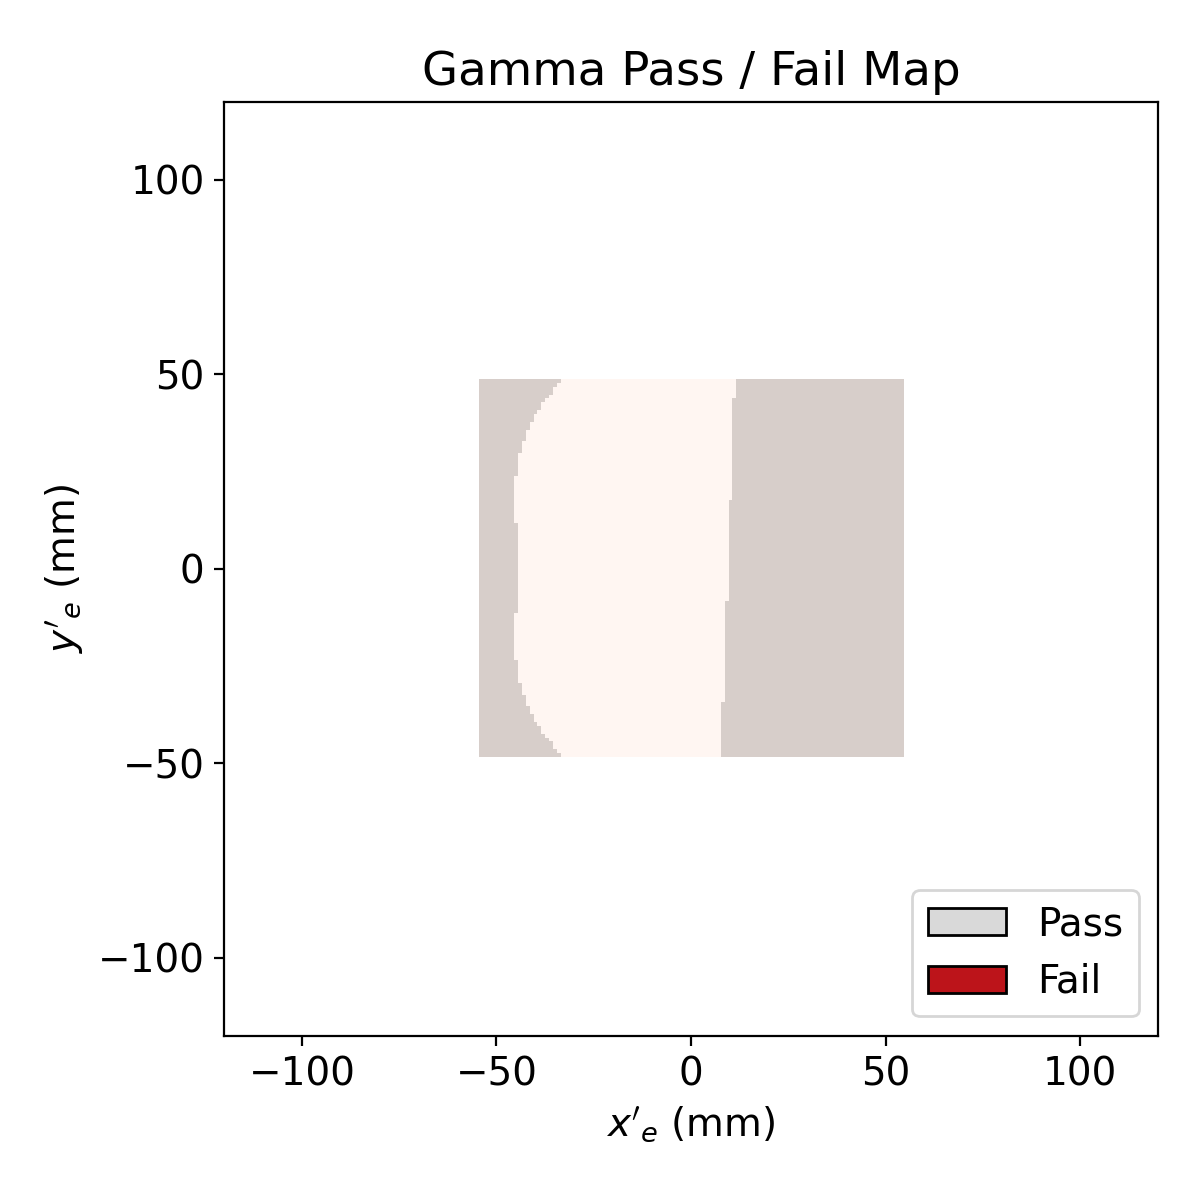
\includegraphics[width=.62\linewidth]{figures/gamma_failures.png}
  \end{tabular}%
  \begin{tabular}{c}
    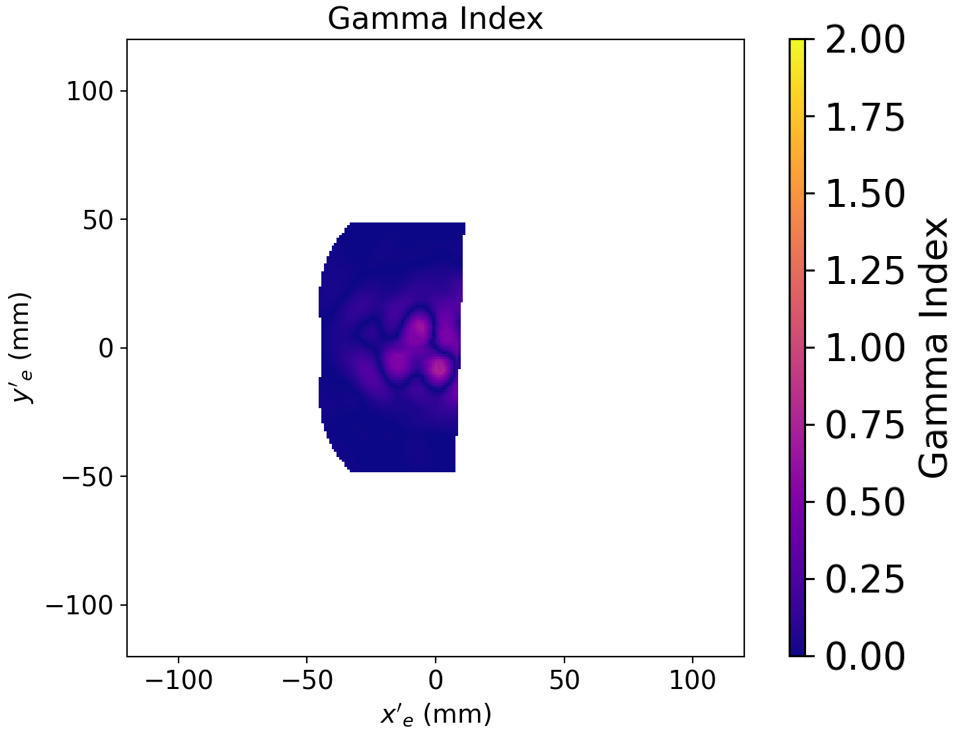
\includegraphics[width=.32\linewidth]{figures/gamma_index_with_colorbar.png} \\
    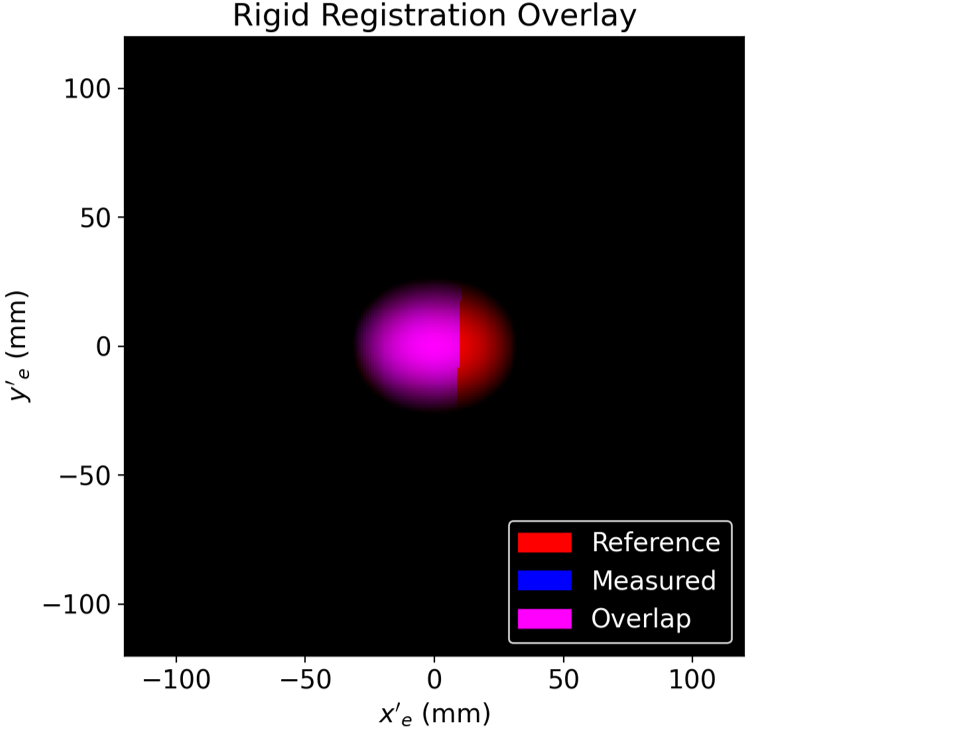
\includegraphics[width=.32\linewidth]{figures/registration_nocolorbar.png} \\
  \end{tabular}
  \begin{tabular}{c}
    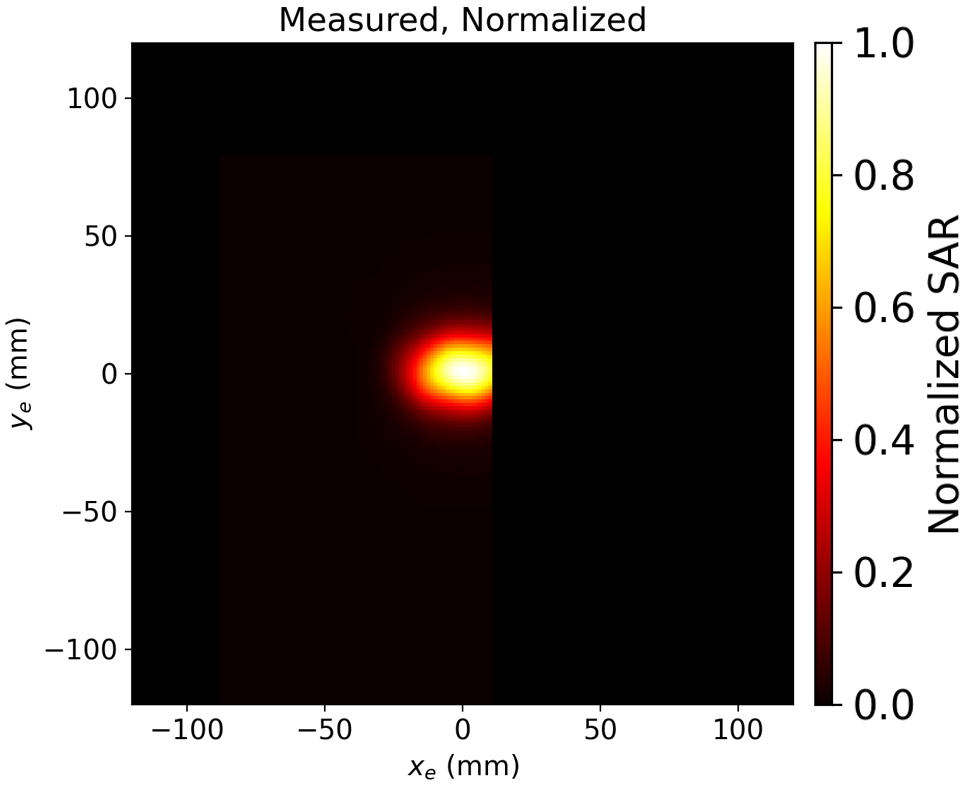
\includegraphics[width=.45\linewidth]{figures/measured_with_colorbar.png}
  \end{tabular}%
  \begin{tabular}{c}
    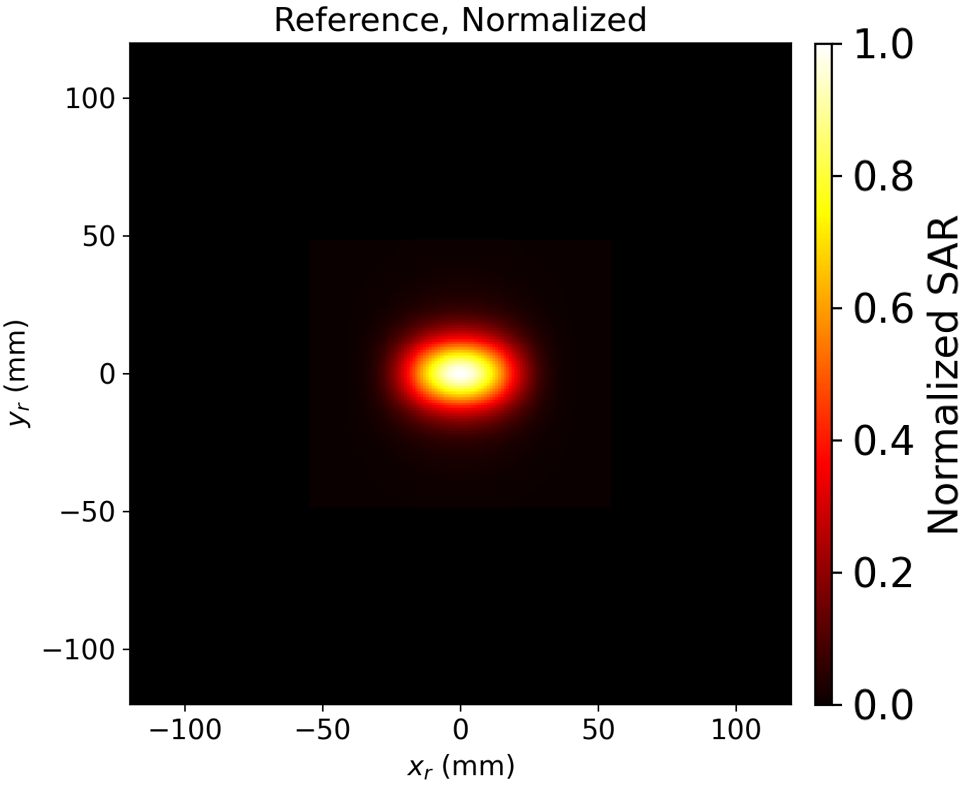
\includegraphics[width=.45\linewidth]{figures/reference_with_colorbar.png}
  \end{tabular}
  % \caption*{}
\end{figure}
\end{document}

% \maketitle
% \thispagestyle{empty}

% \section*{Background}

% This report documents the validation of a measured spatially-averaged SAR (sSAR) pattern compared to a reference distribution. A reference software implementation is provided, where a measured sSAR distribution is uploaded and the input parameters are chosen (antenna type, frequency, distance, and averaging mass). The software evaluates the Gamma match and determines whether the sSAR distribution is compliant, according to the criteria. The software also creates plots to show the measured and reference SAR distributions, the registration overlay, the gamma index map and the pass/fail map.

% Validation of spatial SAR distributions is performed using the Gamma method developed by Low and Dempsey~\cite{low-dempsey} to compare measured spatial SAR distributions, $sSAR_{en}(x_e,y_e)$, with corresponding reference distributions, $sSAR_{rn}(x_r,y_r)$, each normalized to its peak value. The Gamma method combines two criteria, SAR magnitude difference and spatial distance-to-agreement, combining these two dimensions (after normalization by their respective tolerances $\Delta D$ and $\Delta d$) into a single Euclidian distance norm, $\Gamma$, which is used to identify corresponding points:


% $sSARen(x_e,y_e)$ and $sSARrn(x_r,y_r)$ are both extracted at the boundary between the phantom shell and lossy medium. Before normalization, masking is performed to select only those values above 0.1 W/kg or twice the noise floor of the system, whichever is lower. A rigid transformation is first applied to the reference coordinates ($x_r$, $y_r$) to get the registered reference coordinates ($x'_r$, $y'_r$) on a 1~mm regular grid that optimally matches the evaluated distribution to the reference distribution. For each point ($x_e$, $y_e$) on $sSAR_{en}$, all points ($x'_r$, $y'_r$) are searched to identify the corresponding point with the minimal Gamma index. The validation is considered successful if $\Gamma (x_e,y_e)~\leq~1.0$ for all points.

% \bibliographystyle{ieeetr}
% \bibliography{sample}

% \FloatBarrier
% \clearpage
% \newpage

% \begin{table}[htpb] \centering
% \begin{tabular}{cc|cc}
% \multicolumn{2}{c|}{\textbf{Output}} & \multicolumn{2}{c}{\textbf{Gamma Parameters}} \\
% \textbf{Result} & \textbf{Pass Rate (\%)} & \boldmath{$\Delta D$} & \boldmath{$\Delta d$} \\\hline
% \passfail & \passrate & \deltadose & \deltadist \\
% \end{tabular}
% \label{tab:meas-params}
% \end{table}
